%%%%%%%%%%%%%%%%%%%%%%%%%%%%% Define Article %%%%%%%%%%%%%%%%%%%%%%%%%%%%%%%%%%
\documentclass[11pt]{article}
%%%%%%%%%%%%%%%%%%%%%%%%%%%%%%%%%%%%%%%%%%%%%%%%%%%%%%%%%%%%%%%%%%%%%%%%%%%%%%%

%%%%%%%%%%%%%%%%%%%%%%%%%%%%% Using Packages %%%%%%%%%%%%%%%%%%%%%%%%%%%%%%%%%%
\usepackage{geometry}
\usepackage{graphicx}
\usepackage{amssymb}
\usepackage{amsmath}
\usepackage{amsthm}
\usepackage{empheq}
\usepackage{mdframed}
\usepackage{hyperref}
\usepackage{booktabs}
\usepackage{lipsum}
\usepackage{graphicx}
\usepackage{color}
\usepackage{psfrag}
\usepackage{pgfplots}
\usepackage{bm}
\usepackage{framed}
%%%%%%%%%%%%%%%%%%%%%%%%%%%%%%%%%%%%%%%%%%%%%%%%%%%%%%%%%%%%%%%%%%%%%%%%%%%%%%%

% Other Settings

%%%%%%%%%%%%%%%%%%%%%%%%%% Page Setting %%%%%%%%%%%%%%%%%%%%%%%%%%%%%%%%%%%%%%%
\geometry{a4paper}

%%%%%%%%%%%%%%%%%%%%%%%%%% Define some useful colors %%%%%%%%%%%%%%%%%%%%%%%%%%
\definecolor{ocre}{RGB}{243,102,25}
\definecolor{mygray}{RGB}{243,243,244}
\definecolor{deepGreen}{RGB}{26,111,0}
\definecolor{shallowGreen}{RGB}{235,255,255}
\definecolor{deepBlue}{RGB}{61,124,222}
\definecolor{shallowBlue}{RGB}{235,249,255}
%%%%%%%%%%%%%%%%%%%%%%%%%%%%%%%%%%%%%%%%%%%%%%%%%%%%%%%%%%%%%%%%%%%%%%%%%%%%%%%

%%%%%%%%%%%%%%%%%%%%%%%%%% Define an orangebox command %%%%%%%%%%%%%%%%%%%%%%%%
\newcommand\orangebox[1]{\fcolorbox{ocre}{mygray}{\hspace{1em}#1\hspace{1em}}}
%%%%%%%%%%%%%%%%%%%%%%%%%%%%%%%%%%%%%%%%%%%%%%%%%%%%%%%%%%%%%%%%%%%%%%%%%%%%%%%

%%%%%%%%%%%%%%%%%%%%%%%%%%%% English Environments %%%%%%%%%%%%%%%%%%%%%%%%%%%%%
\newtheoremstyle{mytheoremstyle}{3pt}{3pt}{\normalfont}{0cm}{\rmfamily\bfseries}{}{1em}{{\color{black}\thmname{#1}~\thmnumber{#2}}\thmnote{\,--\,#3}}
\newtheoremstyle{myproblemstyle}{3pt}{3pt}{\normalfont}{0cm}{\rmfamily\bfseries}{}{1em}{{\color{black}\thmname{#1}~\thmnumber{#2}}\thmnote{\,--\,#3}}
\theoremstyle{mytheoremstyle}
\newmdtheoremenv[linewidth=1pt,backgroundcolor=shallowGreen,linecolor=deepGreen,leftmargin=0pt,innerleftmargin=20pt,innerrightmargin=20pt,]{theorem}{Theorem}[section]
\theoremstyle{mytheoremstyle}
\newmdtheoremenv[linewidth=1pt,backgroundcolor=shallowBlue,linecolor=deepBlue,leftmargin=0pt,innerleftmargin=20pt,innerrightmargin=20pt,]{definition}{Definition}[section]
\theoremstyle{myproblemstyle}
\newmdtheoremenv[linecolor=black,leftmargin=0pt,innerleftmargin=10pt,innerrightmargin=10pt,]{problem}{Problem}[section]
%%%%%%%%%%%%%%%%%%%%%%%%%%%%%%%%%%%%%%%%%%%%%%%%%%%%%%%%%%%%%%%%%%%%%%%%%%%%%%%

%%%%%%%%%%%%%%%%%%%%%%%%%%%%%%% Plotting Settings %%%%%%%%%%%%%%%%%%%%%%%%%%%%%
\usepgfplotslibrary{colorbrewer}
\pgfplotsset{width=8cm,compat=1.9}
%%%%%%%%%%%%%%%%%%%%%%%%%%%%%%%%%%%%%%%%%%%%%%%%%%%%%%%%%%%%%%%%%%%%%%%%%%%%%%%

%%%%%%%%%%%%%%%%%%%%%%%%%%%%%%% Title & Author %%%%%%%%%%%%%%%%%%%%%%%%%%%%%%%%
\title{\textbf{Macroeconomic Theory I \\ Problem Set 4}}
\author{Sankalp Sharma}
\date{\today}
%%%%%%%%%%%%%%%%%%%%%%%%%%%%%%%%%%%%%%%%%%%%%%%%%%%%%%%%%%%%%%%%%%%%%%%%%%%%%%%

\begin{document}
    \maketitle

\noindent \textit{Collect annual time-series data on real, fixed price (ideally) or chained GDP, $Y_t$, current price GDP, $NOMY_t$, current price gross investment, $NOMI_t$, hours worked, $H_t$, and the working age population, $POP_t$ for}

\begin{itemize}
    \item \textit{United States}
    \item \textit{United Kingdom }
\end{itemize}

\noindent \textit{for the same sample period. Ideally, the sample period should be at the latest from 1970 through 2019. It can be a little shorter if one of the countries has a shorter sample period than this available.}
\\
\\    
\textit{Do not attempt to collect data for 2020 or 2021, as they are affected by the pandemic. Check BEA (US), Eurostat, FRED, IMF, OECD, World Bank, and UK-specific sources. Construct the working age population of each country using U.N. Population Estimates data by summing over the population aged 16 through 65 or 20 through 69 or similar.}
\\
\\
\textit{Make the following calculations for each of the countries.}
\\
\\
a. \textbf{Construct a real investment series by calculating} $$I_t = \frac{NOMI_t}{P_t}$$

where $NOMI_t$ is current price investment and $P_t$ is the GDP fixed price deflator. The latter is the ratio of current price to constant price GDP, $$ P_t = \frac{NOMY_t}{Y_t}$$

\textbf{Answer:} I obtain US macroeconomic data from FRED. Specifically, the following variables are used:
\begin{itemize}
    \item $Y_t$: Real GDP, Billions of Chained 2017 Dollars
    \item $NOMY_t$: Nominal GDP, Billions of Dollars
    \item $NOMI_t$: Gross Private Domestic Investment, Billions of Dollars
    \item $P_t$: GDP implicit price deflator, $Index_{2017} = 100$
\end{itemize}

For UK, I obtain data from the Office for National Statistics, the official statistical agency for the United Kingdom. Specifically, the following variables are used: 

\begin{itemize}
    \item $Y_t$: Gross domestic product at market prices: Chained volume measure
    \item $NOMY_t$:  Gross domestic product at current prices
    \item $NOMI_t$: Gross capital formation, Millions of Pounds
    \item $I_t$: Gross capital formation, Millions of Chained 2019 Pounds
    \item $P_t$: GDP implicit price deflator, $Index_{2017} = 100$
    \item 
\end{itemize}

\noindent For UK, I do not construct $I_t$ by dividing $NOMI_t$ by $P_t$ since UK has a \href{https://www.ons.gov.uk/economy/grossdomesticproductgdp/timeseries/ybfu/ukea}{separate deflator} for gross capital formation. I instead use chained value of gross capital formation\footnote{I additionally validated the accuracy of the gross capital formation deflator - $\frac{NOMI_t}{I_t}$ was equal to the deflator value with an upto $10^{-2}$ digits}.
\\ \\ 

\noindent I now plot the real investment to real GDP ratio for both countries from 1970 to 2019.

\begin{figure}[ht]
    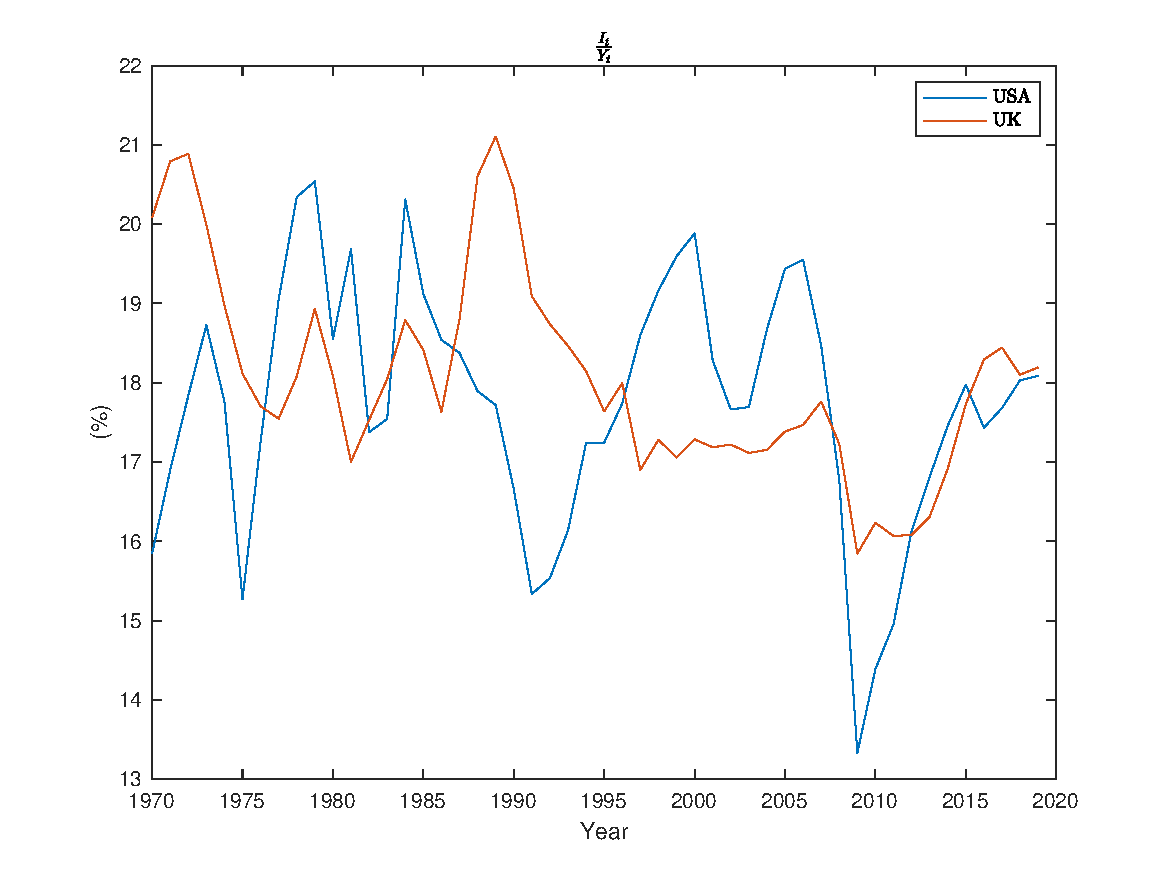
\includegraphics[width=0.7\textwidth]{out/Investment.pdf}
    \centering
\end{figure}

The US investment to GDP ratio has fluctuated between $\sim 13.3\% $ and $20.5\%$ between 1970 and 2019 while the UK investment to GDP ratio has fluctuated between $15.8\%$ to $21.1\%$ in the same period. However, US investment to GDP ratio has shown more volality (as measured by long-run standard deviation) compared to UK.
\\
\\
% QUESTION 1 ENDS HERE

%%%%%%%%%%%%%%%%%%%%%%%%%%%%%%%%%%%%%%%%%%%%%%%%%%%%%%%%%%%%%%%%%%%%

2. \textbf{Use the real investment series, the capital accumulation equation}
$$
K_{t+1}=(1-\delta) K_t+I_t
$$

and follow the numerical method we discussed in class to jointly determine the values of $\delta, K_0$, and $\left\{K_t\right\}_{t=1}^T$. Specifically, you will choose the initial capital stock to satisfy

$$
\frac{K_0}{Y_0}=\left(\frac{1}{10}\right)\left(\sum_{t=1}^{10}\left(K_t / Y_t\right)\right)
$$

given data on initial real GDP, and GDP for the following 10 periods. You will choose the depreciation rate such that sample average depreciation expenditure as a portion of GDP calculated in the data using each country's National Income and Product Accounts (NIPA) data equals that implied by the sample average product of your constructed (real) capital stock and depreciation rate as a ratio of (real) GDP. And use the capital accumulation equation to calculate the time-series of capital stocks over your sample period. You should not use independent sources of information on the depreciation rate, or initial capital stock in making these calculations.
\end{document}